\paragraph{Image acquisition peculiarities} 
    Cells used in this research are growing in 96-well plates. A plate or a microplate in biology is a flat plate with multiple tubes ("wells"). The microscope used in the experiments takes photos of the well plate in random locations. The reason for that hides in the focusing settings of a  microscope. To get a reasonably good not blurry photo a microscope has to focus on a specific location of the plate, the choice of this location however happens automatically, therefore the location of the focus is random (see Figure \ref{fig:random-dic}). 
    
    It might be problematic in the following sense: photos takes in such manner do not gurantee that the focus will land in distinct spots all the time. Meaning that some cells present in one of the photos might appear in the other ones as well. Since the photos are high-resolution they weil be first splitted into crops of size $256 \times 256$ each during the preprocessing. And it might happen that same cells might appear in several crops. That is why after the split of the image data between train, test and validation sets it might also happen that the same set of cells will once land in the train set and another time in the validation set, which will lead to a not completely fair and representative validaiton metrics during training.
    
    In order to overcome this problem a much more expensive equipment is needed. Since in this case it doesn't bring too huge problems except for the fact that validation metrics might be lower than they should have been, there was no need to purchase a more expensive equipment.   
    
    \begin{figure}[htb]
        \begin{center}
            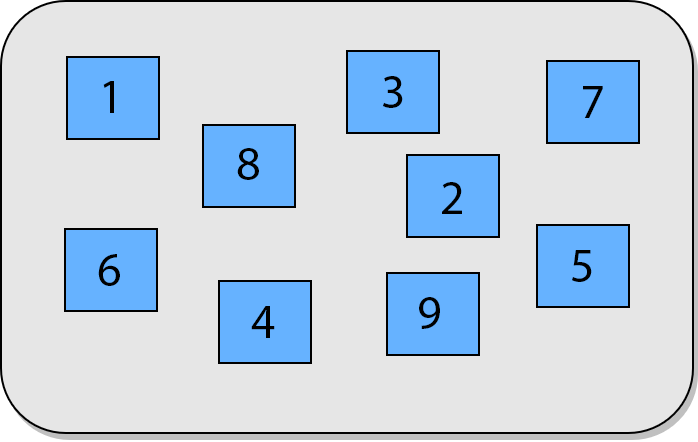
\includegraphics[width=0.3\linewidth]{bilder/dic-random.png}
            \caption{Way in which photos of the well-plate were taken}\label{fig:random-dic}
        \end{center}
    \end{figure}    
\paragraph{Crops combination technique}\label{par:crops-combination}
    Due to the restricted amount of memory on the GPU deep learning models cannot have a high-resolution image as their input in the scope of this research. Yet this is also not obligatory: as the image contains dozens of cells within it, its processing can be limited to a crop of a smaller size. After the model has predicted fluorescence signal for each of the crops, output fluorescence images can be combined together to form a high-resolution image again. In this thesis the architecture of the model assumes an input size of $(256, 256)$ or more specifically $(None, 1, 256, 256)$, where the first dimension is responsible for the batch size and the second one states that the input is a 1-channel image. 

There are several ways of how one can split the image, the easiest approach would be to use a sliding window of size $w$. This algorithm is depicted in Figure \ref{fig:sliding-window}. A small window starts sliding the image from the upper left to the lower right corner with step size $s$ feeding the selected crops into a deep learning model. From the output of the model only a center part of such a crop is accepted to form a full fluorescence image. Border size $b$ in this case is the size of the edges of the crop that are not accepted from the predictions of the deep learning model.

Accepted areas from each of the crops have to follow each other without any space in between. In oder to achieve that if the border size has been defined in advance, one has to set the step size to in the following way:
\begin{equation}
  s = w - 2 * b
\end{equation}
When step size $s$ is equal to window size $w$, there is no overlap between the windows.

\begin{figure}[H]
	\begin{center}
		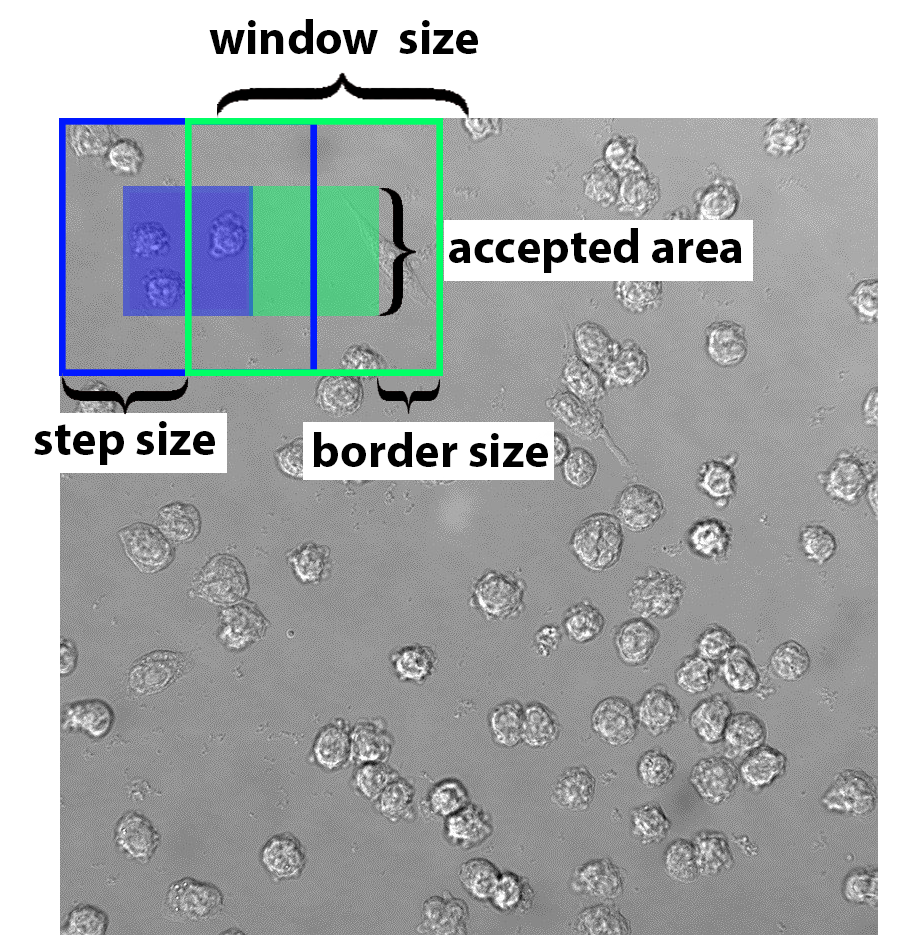
\includegraphics[width=0.3\linewidth]{bilder/sliding-window.png}
		\caption{Sliding window approach for fluorescence prediction}\label{fig:sliding-window}
	\end{center}
\end{figure}
The reason why the full prediction is not accepted to form the output lies in the following: trained models are less accurate on the borders of the crops rather than in the center. Most of the times there are cells on the borders of the crops that were sliced and therefore it might be impossible to make a good prediction for them just due to the lack of input information. Therefore, the step size has to be smaller than the window size, so that the windows are overlapping and for each prediction we use only the image center and are allowed to ignore predictions on the border (see the comparison between different border sizes in Figure \ref{fig:crops-combination}). This is discussed in more detail in Section [TODO reference the section]. Such an approach helps to reduce the effect of grid visibility on the image composed of many small crops. This can be seen in the left part of Figure 5 as opposed to the non-visible borders in the same Figure on the right. This would of course take more time to created the predictions, however, the speed is less crucial in comparison to the accuracy of the predictions.

\begin{figure}[htb]
	\begin{center}
		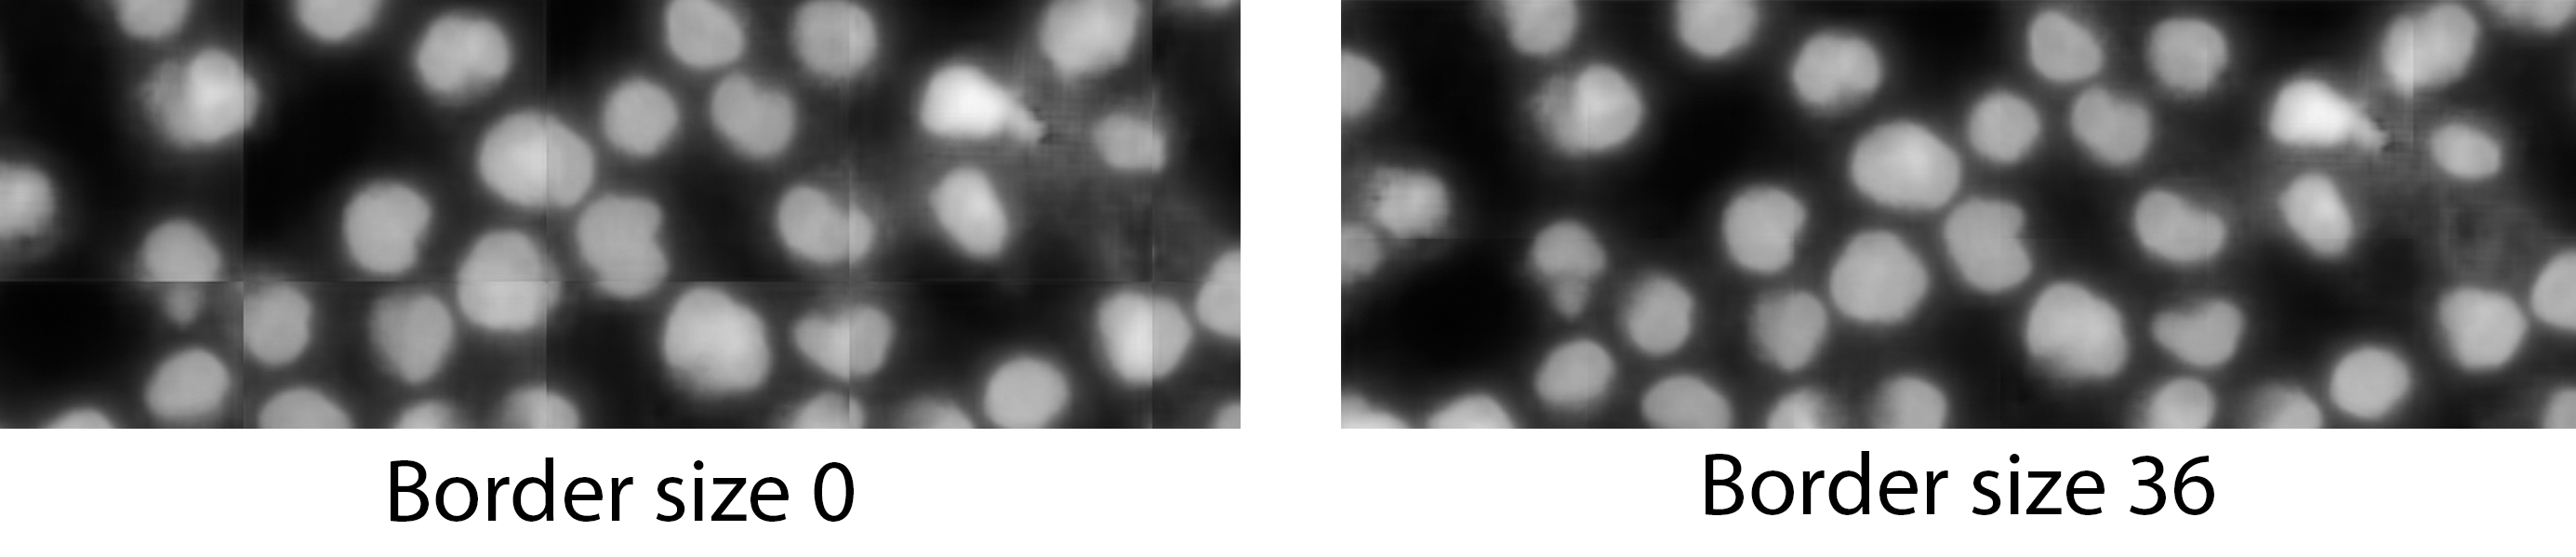
\includegraphics[width=\linewidth]{bilder/crops_combination/crops-combination.png}
		\caption{Difference of overlap between predictions on the resulting image}\label{fig:crops-combination}
	\end{center}
\end{figure}